\chapter{Kiểm tra kết quả}

Bất kỳ một sản phẩm nào đều cần phải được kiểm tra trước khi công bố, luận văn này cũng không phải là một ngoại lệ. Để đảm bảo chất lượng được đánh giá một các khách quan nhất, một hệ thống testcase với các loại tình huống được phân bổ một cách khoa học sẽ được đưa ra, chỉnh sửa cho phù hợp với 2 bài toán của luận văn là Kiểm tra kiểu và Suy luận kiểu và chạy thử để đưa ra kết quả. Tuy nhiên, để chạy được các giải pháp của luận văn, cần chọn một trình dịch ngược sẵn có và chỉnh sửa, hiện thực giải pháp trên đó. Trình dịch ngược được chọn là Boomerang như đã trình bày ở phần \ref{sec:whyboom}. Phần đầu của chương này sẽ trình bày các thiết lập cần thiết trên Boomerang để hiện thực giải pháp cho kiến trúc máy 8051 như phần giới hạn của chương trình. Phần tiếp theo đề ra phương pháp kiểm thử bao gồm cách lập testcase và kết quả chạy thử testcase trên các giải pháp.

\section{Thiết lập Boomerang}

\label{sec:boomchange}
Ở phần \ref{sec:whyboom}, một bảng đánh giá các trình dịch ngược hiện tại đã được đưa ra để lựa chọn trình dịch ngược phù hợp nhất để hiện thực giải pháp và Boomerang đã được chọn vì có số điểm ở các tiêu chí cao nhất. Tuy nhiên, để hiện thực các thuật toán của luận văn, cần có các chỉnh sửa sau:
\begin{itemize}
	\item Xử lý để Boomerang giữ được tên biến được người dùng tự khai báo. Vì bản thân Boomerang là một trình dịch ngược từ mã máy, nên nó chỉ xử lý dữ liệu dưới dạng thanh ghi, các thanh ghi này phải được định nghĩa trước trong file đặc tả của từng kiến trúc máy.
	\item Chỉnh sửa giai đoạn sinh mã của Boomerang. Các giải pháp đưa ra trong luận văn đều có kết quả cuối cùng là một danh sách các UnionDefine tương ứng với những union tìm thấy được. Để đưa các UnionDefine này thành các cấu trúc union ở mã đầu ra, cần phải có một số thay đổi ở phần sinh mã của Boomerang
\end{itemize}
Các thay đổi này sẽ	 lần lượt được trình bày ở các phần dưới.

\subsection{Thay đổi cơ chế quản lý tên dữ liệu của Boomerang}

Vì ở mức độ mã máy, dữ liệu chỉ được lưu ở các thanh ghi cố định hoặc vùng nhớ được truy xuất bằng địa chỉ nên Boomerang không có cơ chế xử lý các biến được người dùng tạo ra ở mã assembly. Tuy nhiên, Boomerang vẫn có cơ chế để giữa được tên các thanh ghi đó ở đoạn mã đầu ra, nên cần tìm hiểu về cơ chế này và chỉnh sửa để nó linh hoạt chấp nhận tất cả các tên biến khác chứ không chỉ riêng tên thanh ghi.

\subsubsection{Phương thức lưu trữ tên thanh ghi của Boomerang}
Khi chuyển đổi từ mã assembly sang mã trung gian, Boomerang sẽ dùng một class con của \textit{Expr} để biểu diễn thanh ghi. Cụ thể là class \textit{Location}, và gọi phương thức static của class \textit{Location} là \textit{Location::regOf(int num)}, phương thức này cần được truyền vào một con số đại diện cho thanh ghi. Cặp số - tên thanh ghi này được lưu vào một từ điển, để sau này khi thực hiện phân tích xong thì sẽ chuyển lại từ thanh ghi thành biến cục bộ.

Trong phần giải mã từ mã assembly sang mã trung gian, có một hàm để map giữa tên thanh ghi và con số đại diện cho nó, đó là hàm \textit{map\_sfr(string name)} được thể hiện ở đoạn mã \ref{list:listmapsfr}.
\begin{lstlisting}[caption={Một số phần mã trong hàm map\_sfr},label={list:listmapsfr},language=c++]
if (name == "R0") return 0;
else if (name == "R1") return 1;
else if (name == "R2") return 2;
...
else return -1;

\end{lstlisting}

Sau khi trải qua các quá trình phân tích và đến giai đoạn in ra mã đầu ra, trình dịch ngược sẽ gọi hàm \textit{getRegName} trong class \textit{FrontEnd} để trả lại tên ban đầu của thanh ghi. Hàm này được trình bày ở đoạn mã \ref{list:listgetregname}. Trong hàm \textit{getRegName}, Boomerang sẽ lấy từ điển tên thanh ghi - số đại diện được quy định sẵn trong đặc tả của các kiến trúc máy, tìm tên thanh ghi tương ứng với con số đó và trả về.
\begin{lstlisting}[caption={Phần mã trong hàm getRegName},label={list:listgetregname},language=c++]
std::map<std::string, int, std::less<std::string>>::
																				iterator it;
for (it = decoder->getRTLDict().RegMap.begin();	 it != 										
	decoder->getRTLDict().RegMap.end(); it++)
	if ((*it).second == idx) 
		return (*it).first.c_str();
return NULL;
\end{lstlisting}


Như vậy, có thể thấy với các tên biến không được quy định trước, hàm \textit{map\_sfr} sẽ trả về giá trị \textbf{-1}, và vì giá trị \textbf{-1} sẽ không có trong từ điển của kiến trúc máy, nên hàm \textit{getRegName} sẽ trả về \textbf{NULL}, dẫn đến trình dịch ngược sẽ bị lỗi runtime và dừng ngay lập tức.\\

%lấy mã Boomerang ban đầu về, hiện kết quả khi sử dụng biến đầu vào

\subsubsection{Chỉnh sửa phương thức trên để chấp nhận tên biến tự khai báo}
Vì số lượng tên biến là rất nhiều, nên giải pháp thêm mới các tên biến vào từ điển được quy định sẵn là không khả thi, mà phải có cách để trình dịch ngược linh động hơn, chấp nhận bất kỳ các tên nào được sử dụng trong mã assembly. Giải pháp đưa ra là ngoài việc sử dụng từ điển thanh ghi được quy định sẵn, một bảng tên biến sẽ được lập thêm, thành phần bao gồm các cặp tên biến - số đại diện. Trong giai đoạn giải mã, khi hàm \textit{map\_sfr} được gọi, nếu tên truyền vào nằm trong các thanh ghi đã quy định sẵn, thay vì trả về giá trị \textbf{-1} thì ta sẽ tạo ra một giá trị random và đưa chúng vào bảng tên biến ở trên. Ngoài ra, còn có một đoạn mã kiểm tra biến được sử dụng đã được khai báo chưa (ngoại trừ một số biến đặc biệt được tự sinh). Hàm \textit{map\_sfr} nâng cấp được trình bày trong đoạn mã \ref{list:listmapsfrnew}.\\
\begin{lstlisting}[caption={Phần mã mới được bổ sung trong hàm map\_sfr},label={list:listmapsfrnew},language=c++]
bool isDefined = false;
map<char*, AssemblyArgument*>::iterator it;
for (it = replacement.begin(); it!=replacement.end()
		; it++){
	if(strcmp((*it).first, name.c_str()) == 0 ){
		isDefined = true;
		break;
	}
}
if (isDefined || name.find("specbits") != string::npos ){
	if (symbolTable->find(name) 
		== symbolTable->end()){
		bool existed = false;
		int num;
		do{
			num = std::rand()%200+31;
			map<string, int>::iterator it;
			for (it = symbolTable->begin(); it!=symbolTable->end()
				; it++){
				bool cond1 = (*it).second == num;
				bool cond2 = (byteVar != -1 && byteVar>=num);
				bool cond3 = (bit != -1 && bit>=num);
				if (cond1 || cond2 || cond3){
					existed = true;
					continue;
				} else {
					existed = false;
				}	
			}
		} while (existed); 
		(*symbolTable)[name] = num;
		if (name.find("specbits") != string::npos){
			std::cout<<"Name: "<<name<<", "<<num<<endl;
		}	
		return num;
	} else {
		return symbolTable->find(name)->second;
	}
}
else {
	std::cout<<"ERROR: "<<name<<" HAS NOT BEEN DEFINED YET"
			<<endl;
	exit(1);
}
\end{lstlisting}
Tương ứng với sự thay đổi ở hàm \textit{map\_sfr},  ở hàm \textit{getRegName}, ngoài việc dò trong từ điển quy định trước, cần phải bổ sung thêm một đoạn mã để dò trong bảng tên biến. Phần bổ sung này được thể hiện ở đoạn mã \ref{list:listgetregnamenew}.
\begin{lstlisting}[caption={Phần mã mới được bổ sung trong hàm getRegName},label={list:listgetregnamenew},language=c++]
std::map<string,int>::iterator symIt;
for (symIt = decoder->getSymbolTable().begin(); symIt != 
	decoder->getSymbolTable().end(); symIt++){
	if ((*symIt).second == idx){
		return (*symIt).first.c_str();
	}
}
\end{lstlisting}
Như vậy, vấn đề giữ nguyên tên biến được giải quyết mà không ảnh hưởng nhiều tới trình dịch ngược.
%đoạn mã đầu vào assembly và mã đầu ra giữ nguyên được tên biến

\subsection{Thêm trường hợp cấu trúc union vào đoạn sinh mã của Boomerang}

Từ dữ liệu là danh sách các thực thể UnionDefine được rút trích thông qua các giải thuật của luận văn, trình dịch ngược cần phải đưa ra các union tương ứng. Hình \ref{fig:uniondefinemapping} thể hiện việc chuyển đổi của class UnionDefine cho kiến trúc máy 8051 sang cấu trúc union. Các union này được thêm vào danh sách biến toàn cục (global) của chương trình vì chúng có tác dụng trên toàn chương trình chứ không riêng một hàm nào.

\begin{figure}[h!]
\centering
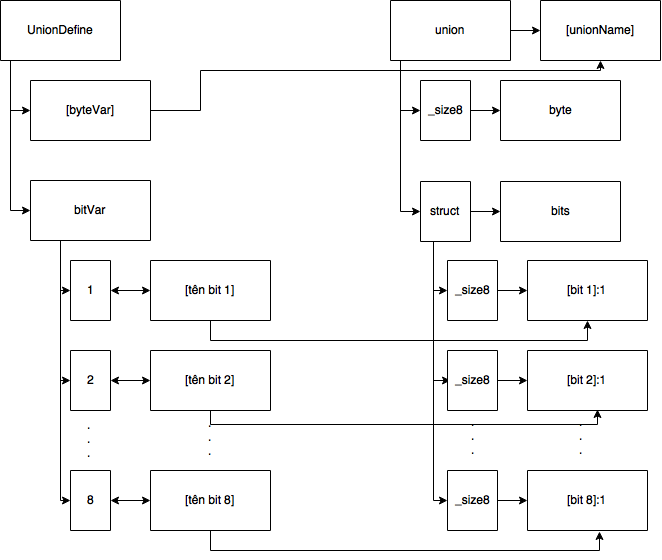
\includegraphics[width=\linewidth]{image/unionDefineMapping}
\caption{Hình minh hoạ việc chuyển đổi từ class UnionDefine cho mã 8051 sang cấu trúc union ở mã đầu ra}
\label{fig:uniondefinemapping}
\end{figure}

Sau khi sinh ra các union như trên, một số thay thế cần được thực hiện trên đoạn mã đầu ra. Cụ thể như sau:
\begin{itemize}
\item Thay thế các biểu thức thể hiện các thành phần của union dưới dạng thanh ghi độc lập thành một biểu thức truy xuất đến union đó. Vì ở giai đoạn giải mã, chưa có thông tin nào về các kiểu union, nên trình dịch ngược sẽ xem tất cả các biến là những đối tượng dữ liệu độc lập với nhau. Sau khi đã trải qua các quá trình phân tích và sinh ra các union, ta cần thay thế để thể hiện rõ mối liên hệ giữa các thành phần của những union đó. Ví dụ như ở đoạn mã \ref{list:listbeforereplacebitvar}, thành phần \textit{TESTSUPS} vẫn đang được xem như là một biến độc lập ở mã đầu ra, và cần phải thay thế nó bằng một truy xuất tới union chứa thành phần \textit{TESTSUPS}, trong trường hợp này là \textit{OPTIONS}. Kết quả của bước thay thế này được thể hiện ở đoạn mã \ref{list:listafterreplacebitvar}.
\begin{lstlisting}[caption={Mã đầu ra trước khi thực hiện các bước thay thế},label={list:listbeforereplacebitvar}, language = c]
a = *OPTIONS;
TESTSUPS = 1;
if (specbits1 == 1){
	...
}
return a;
\end{lstlisting}

\begin{lstlisting}[caption={Mã đầu ra sau khi thực hiện bước thay thế thành phần của union},label={list:listafterreplacebitvar}, language = c]
a = *OPTIONS;
OPTIONS.bits.TESTSUPS = 1;
if (specbits1 == 1){
	...
}
return a;
\end{lstlisting}
\item Thay thế các biểu thức truy xuất trực tiếp một phần của thanh ghi trung gian thành biểu thức truy xuất đến thành phần tương ứng trong kiểu union của thanh ghi đó. Vì một số lý do, có đôi khi lập trình viên không sử dụng tên biến mà dùng biểu thức truy xuất trực tiếp đến một thành phần của thanh ghi trung gian. Ví dụ như trong 8051, người lập trình có thể dùng biểu thức \textit{ACC.1 }để truy xuất tới bit đầu tiên của thanh ghi \textit{ACC}. Với trường hợp này, vì đã có dữ liệu về kiểu union mà thanh ghi trung gian đang mang, các biểu thức dạng này sẽ được thay thế bằng biểu thức truy xuất đến union để đoạn mã đầu ra thống nhất hơn, và có thể tiến hành bước thay thế thanh ghi trung gian được trình bày bên dưới. Lưu ý: trong giai đoạn giải mã, các biểu thức truy xuất trực tiếp này sẽ được thể hiện dưới dạng đặc biệt để dễ dàng nhận biết sau này. Ví dụ như với mã 8051, khi gặp biểu thức \textit{ACC.x}, trình giải mã sẽ chuyển chúng về một thanh ghi đặc biệt có tên là \textit{specbitsx}, với \textit{x} là số thứ tự của bit muốn truy xuất như ở đoạn mã \ref{list:listbeforereplacebitvar}. Tiếp tục ví dụ nêu trên, các truy xuất trực tiếp tới bit của thanh ghi \textit{ACC} cũng được thay thế bằng các biểu thức truy thành phần của union tương ứng. Kết quả là đoạn mã \ref{list:listafterreplacebit}, biến đặc biệt \textit{specbits1} đã được thay thế thành biểu thức \textit{OPTIONS.bits.bit1}.

\begin{lstlisting}[caption={Mã đầu ra sau khi thực hiện bước thay thế truy xuất trực tiếp đến một phần của thanh ghi trung gian},label={list:listafterreplacebit}, language = c]
a = *OPTIONS;
OPTIONS.bits.TESTSUPS = 1;
if (OPTIONS.bits.bit1 == 1){
	...
}
return a;
\end{lstlisting}
\item Thay thế các vị trí sử dụng thanh ghi trung gian bằng union tương ứng. Khi lập trình ở dạng mã assembly, lập trình viên không được phép xử lý các vùng nhớ trực tiếp mà phải thông qua thanh ghi trung gian, tuy nhiên, khi đã chuyển đổi về dạng ngôn ngữ cấp cao, có thể sử dụng trực tiếp tên union trong các câu lệnh mà không cần trung gian qua thanh ghi nữa. Điều này giúp mã đầu ra ngắn gọn, dễ hiểu và trong sáng hơn. Đoạn mã \ref{list:listafterreplaceacc} là kết quả sau khi thực hiện bước thay thế này. Dễ dàng thấy đoạn mã đã gọn hơn rất nhiều do loại bỏ được câu lệnh gán cho biến \textit{a}, và thay thế biến \textit{a} ở câu lệnh return thành truy xuất \textit{OPTIONS.byte}. Vì thực chất \textit{a} đang mang kiểu union \textit{OPTIONS}, nên đoạn mã này hoàn toàn tương đương với đoạn mã ở \ref{list:listafterreplacebit}.

\begin{lstlisting}[caption={Mã đầu ra sau khi thực hiện bước thay thế thanh ghi trung gian},label={list:listafterreplaceacc}, language = c]
OPTIONS.bits.TESTSUPS = 1;
if (OPTIONS.bits.bit1 == 1){
	...
}
return OPTIONS.byte;
\end{lstlisting}
\end{itemize}

Có thể thấy, sau khi thực hiện các bước thay thế mã ở trên, đoạn mã cuối cùng ở hình \ref{list:listafterreplaceacc} đã gọn và dễ đọc hơn rất nhiều so với đoạn mã ban đầu \ref{list:listbeforereplacebitvar}.
\section{Kiểm tra kết quả luận văn trên Boomerang}

\subsection{Hệ thống testcase}
Có các tiêu chí phân loại testcase như sau:
\begin{itemize}
	\item Loại biểu thức được gán vào thanh ghi trung gian (tiêu chí I)
	\item Cách truy xuất một thành phần của thanh ghi (tiêu chí II)
	\item Có vi phạm nguyên tắc sử dụng kiểu union hay không (tiêu chí III)
\end{itemize}
Với mỗi tiêu chí, ta sẽ có các trường hợp sau đây:

Tiêu chí I:
\begin{enumerate}
	\item Một hằng số (I.1)
	\item Giá trị ở một vùng nhớ có địa chỉ là một biến (I.2)
	\item Giá trị ở một vùng nhớ có địa chỉ là một hằng số (I.3)
	\item Giá trị ở một vùng nhớ có địa chỉ là một thanh ghi (I.4)
	\item Giá trị ở một vùng nhớ có địa chỉ là một biểu thức 2 vế. Mỗi vế có thể là một biến byte, một thanh ghi, hoặc một hằng số (I.5)
\end{enumerate}

Tiêu chí II:
\begin{enumerate}
	\item Truy xuất dựa vào một biến đại diện. (II.1)
	\item Truy xuất bằng cấu trúc truy xuất trực tiếp một phần nhỏ hơn của thanh ghi. Ví dụ: \textit{ACC.5} trong mã 8051. (II.2)
\end{enumerate}

Tiêu chí III:
\begin{enumerate}
	\item Không vi phạm nguyên tắc sử dụng kiểu union. (III.1)
	\item Một thành phần của union này được sử dụng khi thanh ghi trung gian đang có kiểu là một union khác. Như ví dụ ở đoạn mã \ref{list:invalid1}, thành phần \textit{TESTUPS} được xác định thuộc union \textit{OPTIONS} thông qua 2 câu lệnh 1 và 2, nhưng sau đó lại được truy xuất ở câu lệnh số 4 khi mà thanh ghi trung gian \textit{ACC} đang mang kiểu union \textit{OPTIONS2}. (III.2)
	\begin{lstlisting}[caption={Đoạn mã có một biến bit thuộc nhiều bộ biến khác nhau},label={list:invalid1}]
	MOV A, OPTIONS ;1
	SETB TESTSUPS ;2
	...
	MOV A, OPTIONS2 ;3
	JB TESTSUPS, BB ;4
	\end{lstlisting}
	\item Tại một thời điểm sử dụng thành phần của một union, thanh ghi trung gian có thể mang nhiều kiểu union khác. Xem ví dụ ở đoạn mã \ref{list:invalid2}, ở câu lệnh cuối cùng, biến \textit{a} có thể mang kiểu union \textit{OPTIONS} hoặc \textit{OPTIONS2}, như vậy không thể xác định được \textit{TESTSDOWNS} thuộc union nào. (III.3)
	\begin{lstlisting}[caption={Đoạn mã ACC có thể mang nhiều giá trị vùng nhớ khác nhau},label={list:invalid2}, language=c++]
	if (TESTSUPS == 1)
		a = *OPTIONS;
	else
		a = *OPTIONS2;
	TESTSDOWNS = 0;
	\end{lstlisting}
	\item Ghi nhận được có hai thành phần cùng thuộc một union và cùng truy xuất đến một vị trí của union đó. Như ở đoạn mã \ref{list:invalid3}, biến \textit{TESTSUPS} và \textit{TESTSDOWNS} đều được sử dụng để truy xuất tới bit đầu tiên của union \textit{OPTIONS}. (III.4)
	\begin{lstlisting}[caption={Đoạn mã có 2 thành phần union cùng truy xuất đến một vị trí vùng nhớ của union đó},label={list:invalid3}]
	...
	#DEFINE TESTSUPS, ACC.1
	#DEFINE TESTSDOWNS, ACC.1
	...
	MOV A, OPTIONS
	SETB TESTSUPS
	...
	MOV A, OPTIONS
	CLR TESTSDOWNS
	\end{lstlisting}
\end{enumerate}

Kết hợp các tiêu chí trên, loại bỏ đi một số trường hợp không thể xảy ra, có tổng cộng 18 trường hợp cần kiểm thử. Hầu hết mỗi trường hợp sẽ có một testcase đại diện, nhưng với một số trường hợp phức tạp sẽ có nhiều testcase hơn. Bảng 5.1 thể hiện việc phân bổ testcase theo các trường hợp của các tiêu chí.
\begin{table}[h!]
	\centering
	\begin{tabular}{ |p{0.7cm}| p{2cm}| p{2cm}| p{2cm}| p{5cm}|}
		\hline
		
		STT & Tiêu chí I & Tiêu chí II & Tiêu chí III & Mã testcase\\
		\hline
		1 & 1 & 1 & 1 &TC001\\
		\hline
		2 & 1 & 2 & 1 &TC002\\
		\hline
		3 & 2 & 1 & 1 &TC003\\
		\hline
		4 & 2 & 2 & 1 &TC004\\
		\hline
		5 & 3 & 1 & 1 &TC005\\
		\hline
		6 & 3 & 2 & 1 &TC006\\
		\hline
		7 & 4 & 1 & 1 &TC007, TC019, TC024\\
		\hline
		8 & 4 & 2 & 1 &TC008\\
		\hline
		9 & 5 & 1 & 1 &TC009\\
		\hline
		10 & 5 & 2 & 1 &TC010, TC020\\
		\hline
		11 & 2-3& 1 & 2 &TC011\\
		\hline
		12 & 4-5 & 1 & 2 &TC012\\
		\hline
		13 & 2-3 & 1 & 3 &TC013, TC023\\
		\hline
		14 & 2-3 & 2 & 3 &TC014\\
		\hline
		15 & 4-5 & 1 & 3 &TC015, TC021, TC022\\
		\hline
		16 & 4-5 & 2 & 3 &TC016\\
		\hline
		17 & 2-3 & 1 & 4 &TC017\\
		\hline
		18 & 4-5 & 1 & 4 &TC018\\
		\hline
	\end{tabular}
	
	
	\label{table:table2}
	\caption{Bảng phân bổ các testcase theo từng trường hợp của các tiêu chí}
\end{table}
\subsection{Kết quả chạy thử}

Tuỳ thuộc vào bài toán cần kiểm tra kết quả là gì, các testcase sẽ được điều chỉnh cho phù hợp. Với bài toán Kiểm tra kiểu, phần khai báo của testcase phải cung cấp thông tin về các union theo mẫu quy định, còn bài toán Suy luận kiểu thì không cần. Tuy nhiên nội dung của của các testcase được giữ nguyên để đảm bảo kết quả chạy ra của hai bài toán là như nhau. Kết quả chạy thử các testcase trên từng bài toán được thể hiện ở bảng 5.2

\begin{table}[h!]
	\centering
	\begin{tabular}{ |p{0.7cm}| p{3cm}| p{5cm}| p{5cm}|}
		\hline
		
		STT & Tiêu chí & Bài toán Kiểm tra kiểu & Bài toán Suy luận kiểu\\
		\hline
		1 & Số testcase đúng & 15/24 & 24/24\\
		\hline
		2 & Các testcase bị sai &TC009, TC010, TC012, TC015, TC016, TC018, TC020, TC021, TC022 &\\
		\hline
		3 & Nguyên nhân bị sai & Do phương pháp phân tích dữ liệu được sử dụng không xử lý được hết các trường hợp biểu thức quy định địa chỉ vùng nhớ gán cho thanh ghi trung gian, nên những testcase mà biểu thức này có hai toán hạng sẽ bị sai & \\
		\hline
	\end{tabular}
	
	
	\label{table:table3}
	\caption{Bảng kết quả chạy thử testcase cho hai bài toán}
\end{table}
Như vậy, có thể thấy với bài toán Kiểm tra kiểu, có nhiều testcase cho ra kết quả sai, còn bài toán Suy luận kiểu thì tất cả các trường hợp đều chính xác. Điều này đã được dự báo trước vì kỹ thuật phân tích sử dụng trong bài toán Kiểm tra kiểu còn nhiều hạn chế.\\

